\documentclass{article} %[letterpaper,11pt]
%\usepackage[latin1]{inputenc}
\usepackage{graphicx}
\usepackage{wrapfig}
%\usetikzlibrary{shapes,arrows}

\usepackage{amsmath}

\newcommand{\code}[1]{\texttt{#1}}
\renewcommand\refname{5  \hspace{4 mm}References}

\begin{document}

\title{CS 867: Program 2}
\date{October 2, 2013}
\author{Carmen St.\ Jean}

\maketitle

\section{Introduction}
Designing a symbol set where each symbol is easily findable in a random field of the others can be a difficult task, especially when the symbol set is larger.  Treisman and Gelade found that we process certain features -- such as color, orientation, and form -- pre-attentively and in parallel \cite{treisman80}.  They also concluded that more focused attention is needed to distinguish an object on two or more features.  Therefore, we have taken these ideas into consideration while endeavoring to design and evaluate a symbol set with maximum findability.

In order to take advantage of the pre-attentive processing, the symbols used in this experiment, seen in Figure~\ref{fig:symbolSet}, were given at least one unique feature.  In particular, each symbol has its own distinctive color.  Colors that tend to be easily named (e.g., ``blue," ``pink," ``black") were preferred over colors that may have more ambiguous names (e.g., ``aquamarine," ``teal," ``cerulean").  Each combination of form and orientation is unique; some forms are repeated but with a different orientation.

\begin{figure}[htb]
\centering
	
\includegraphics[width=8cm]{images/symbolset.eps}
	\caption{The symbol set developed for the experiment.}
	\label{fig:symbolSet}
\end{figure}



\begin{wrapfigure}[6]{r}{0.35\textwidth}
\centering
	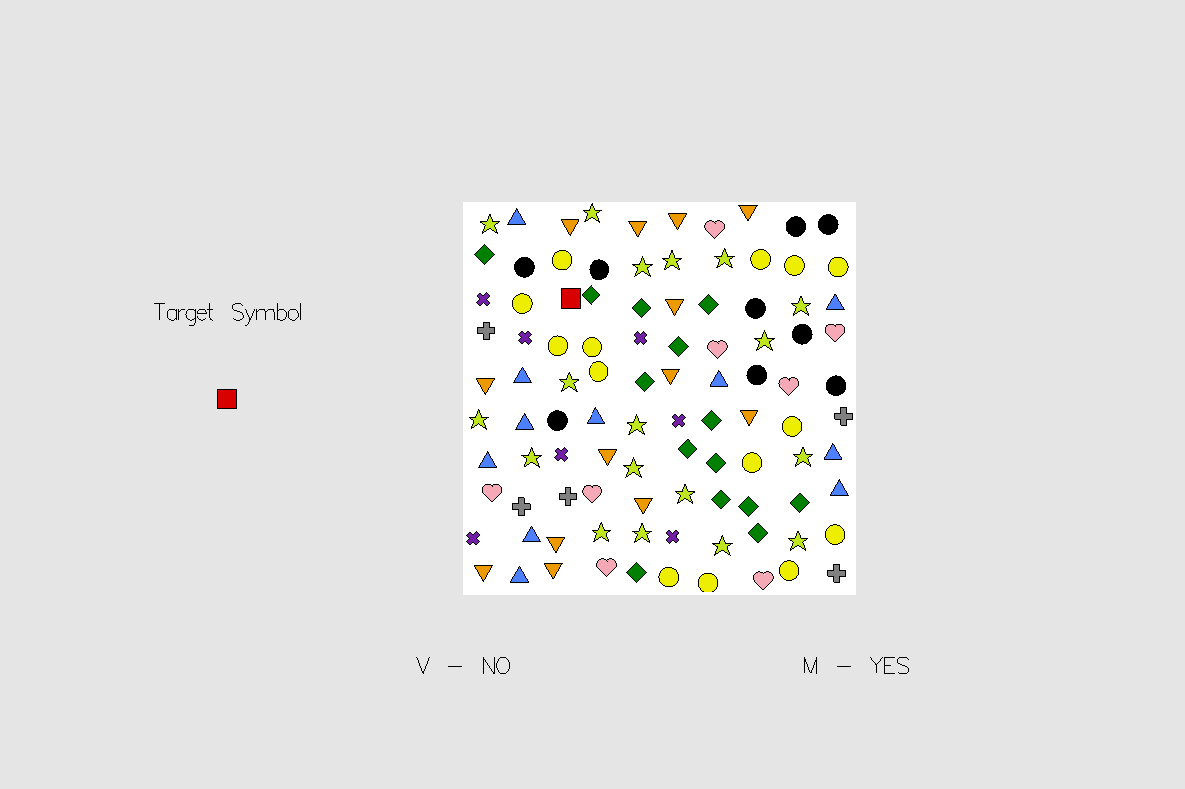
\includegraphics[width=0.35\textwidth]{images/example.eps}
	\caption{An example of a trial.}
	\label{fig:trialExample}
\end{wrapfigure}

\section{Method}

The task of the subject in this experiment was to indicate whether or not a specified target symbol was present in a jittered grid of 100 symbols.

\subsection{Stimuli}

The symbols were drawn using OpenGL on a 10 cm by 10 cm white grid, as seen in Figure \ref{fig:trialExample}.  The grid was in a 30 cm by 10 cm, gray rectangle.  Each individual symbol fit into a 5 mm square, with its position randomly jittered within its 10 mm square space.  No symbols overlapped each other.

Each trial had a target symbol, drawn to the left of the grid and labeled as ``Target."  There were two types of trials: ``Target Trials" and ``Blank Trials."  Target Trials consisted of one target symbol and 99 distractor symbols chosen randomly from the set of nine non-target symbols.  The location of the target symbol in the grid was randomized.  Blank Trials consist of 100 symbols chosen randomly from the set of nine non-target symbols.

\subsection{Procedure}

Trials were given in blocks of 30, with the same target symbol for all trials in the block.  Of those 30 trials, 15 trials were Target Trials and 15 trials were Blank Trials.  The ordering of these trials within the blocks was randomized.  A trial block was given for each of the ten target symbols, making for 300 total trials.  There was approximately one second of blank screen between the trials within a block.  Between blocks, there were approximately five seconds of blank screen to indicate a different symbol would be the target on the next trial.

The experiment began with a ``splash screen" telling the user to press the space-bar to begin.  Instructions for which keys to press for responses were also shown on the splash screen and continued to be displayed throughout the experiment.  When the subject pressed space, a trial appears with a grid of 100 symbols and a target symbol to the left.  The subject then typed the ``M" to indicate the target was perceived as present in the grid of symbols and ``V" if the target seemed to be absent.  Responses were timed.


\begin{wraptable}[11]{r}{0.45\textwidth}
	\resizebox{0.45\textwidth}{!}{%
	\centering
	\begin{tabular}{| r | c | c | c | }
		\hline
		\textbf{Symbol} & \textbf{Target} & \textbf{Blank} & \textbf{All}  \\ \hline
		0   & 0.5907 & 0.9011 & 0.7459 \\ \hline
		1   & 0.7097 & 0.9681 & 0.8389 \\ \hline
		2   & 0.9253 & 1.8779 & 1.4016 \\ \hline
		3   & 0.8111 & 1.8682 & 1.3396 \\ \hline
		4   & 0.6674 & 1.1696 & 0.9185 \\ \hline
		5   & 0.8735 & 2.8849 & 1.8792 \\ \hline
		6   & 1.2615 & 3.2849 & 2.2732 \\ \hline
		7   & 0.7505 & 1.9641 & 1.3573 \\ \hline
		8   & 1.2015 & 2.7635 & 1.9825 \\ \hline
		9   & 0.7175 & 1.6081 & 1.1628 \\  \hline
		 All & 0.8509 & 1.9291 & 1.3900 \\  \hline
	\end{tabular}}
	\caption{Average response times of the different trial types in seconds.}
	\label{tab:averages}
\end{wraptable}

\subsection{Subject}

The subject was one woman, a graduate student at the University of New Hampshire.  Her age was 25 and her vision had been corrected to 20-20 with glasses.  The subject's eyes were approximately 45 cm from the screen.

\section{Results}

The target symbol, target presence, correctness of the response, and the response time were recorded for each of the 300 trials.  

\subsection{Error}

The subject made correct responses in identifying whether or not the target was present in all 300 trials of the experiment, so there was no error.

\subsection{Response Time}

Averages were calculated for each individual target for its 15 Target Trials and 15 Blank Trials, as well as an average taken across all 30 trials.  Additionally, the averages of all 150 Target Trials, all 150 Blank Trials, and all 300 total trials were taken.  These values can be found in Table \ref{tab:averages} and in illustrated form in Figure \ref{fig:averages}

\begin{figure}[htb]
	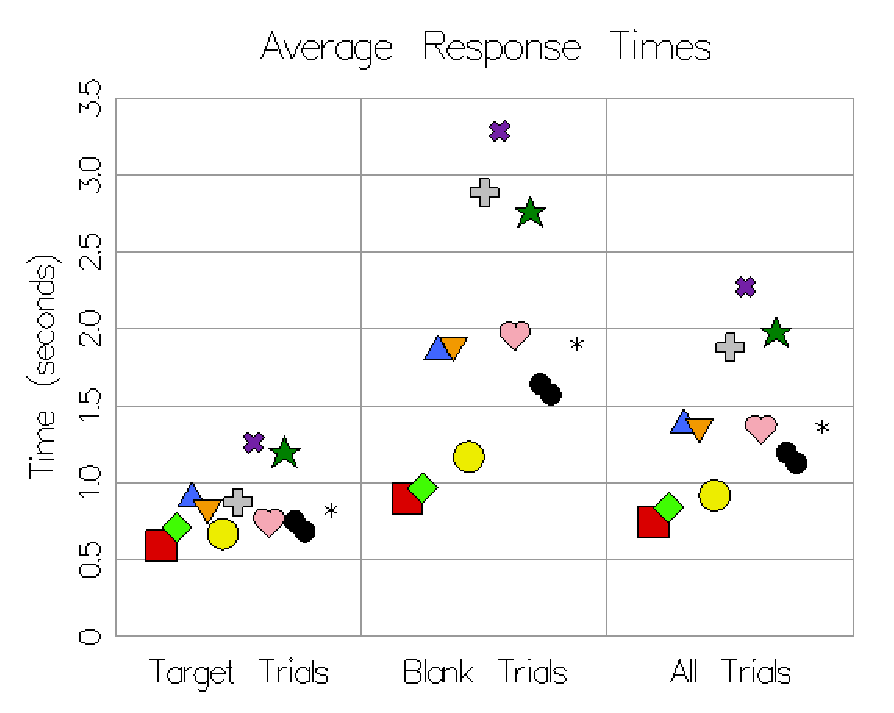
\includegraphics[width=12cm]{images/average-response-times.eps}
	\caption{Plot of average response times of the different trial types by symbol in seconds.  The asterisk (*) indicates the average of all symbols in the experiment.}
	\label{fig:averages}
\end{figure}

\section{Discussion}

Figure~\ref{fig:averages} emphasizes the effectiveness of different symbols.  Symbols 5 (gray plus-sign), 6 (purple X), and 8 (green star) seem to be least findable because they had high average times, especially for Blank Trials.  This could be because these symbols were easily confused for each other, with each of them having at least four protruding parts.  These colors are also either lower in or completely lacking in saturation, which may have made them stand out less.  The symbols which had the lowest average times were symbols 0 (red square), 1 (green tilted square), and 4 (yellow circle).  These symbols were most findable perhaps because they are quite simple in form and their colors are very vivid.

\begin{wraptable}[20]{r}{0.33\textwidth}
	\resizebox{0.33\textwidth}{!}{%
	\centering
	\begin{tabular}{| r | r | }
		\hline
		\textbf{Symbol} & \textbf{\% Increase} \\ \hline
		0	&  52.6\\ \hline
		1	&  36.4 \\ \hline
		2	& 103.0\\ \hline
		3	& 130.3 \\ \hline
		4	&  75.2 \\ \hline
		5	& 230.3 \\ \hline
		6	& 160.4 \\ \hline
		7	& 161.7 \\ \hline
		8	& 130.0 \\ \hline
		9	& 124.1 \\ \hline
		ALL	& 126.7 \\ \hline
	\end{tabular}}
	\caption{Percent increase in average response time from Target Trials to Blank Trials.}
	\label{tab:increase}
\end{wraptable}

Response time averages were significantly larger for Blank Trials than for Target Trials.  This was as expected, as a Target Trial ends as soon as the target is spotted, which may be immediately if the target ``pops out" from the others.  On the other hand, a Blank Trial requires that the subject's eyes look at all 100 symbols before the subject can declare with confidence that the target truly is absent.  However, the average response time increased from Target to Blank trials much more for some targets than others.  In Table~\ref{tab:increase}, we have calculated the percentage increased, as follows, for each target:

\begin{equation*}
x = \frac{t_{blank} - t_{target}}{t_{target}}
\end{equation*}

Table~\ref{tab:increase} shows that symbols 0 (red square), 1 (green tilted square), and 4 (yellow circle) had relatively low increases from Target Trials to Blank Trials.  A low increase is preferrable, meaning these three symbols were particularly effective.  Symbol 5 (gray plus-sign) had a high increase, meaning this symbol is perhaps less effective.


There were no errors and the average response times -- found to be between 0.5 and 3.5 seconds -- were all reasonably low.  This leads to the conclusion that this symbol set is reasonably effective, however that is not to say there is no room for improvement.  It seems that color was more significant than shape, though more work would have to be done to verify this.  Altering the colors and/or shapes of the more poorly performing symbols -- 5 (gray plus-sign), 6 (purple X), and 8 (green star) -- might be recommended before putting this symbol set into practical use.

\bibliographystyle{plain}

\bibliography{carmen-prog2-writeup}

\end{document}

